\subsection{High concentrations of phosphatidylethanolamine}

	To avoid the undesired $Xv$ and $\mu$ underestimation, a less realistic scenario was considered. An extra carbon source was put in excess in the feed medium. We select the phosphatidylethanolamine ($PE$) because it was already introduced in the $Recon3D$ medium, do to the incapacity of this GEM to growth without this (or similar) metabolite, and it is an usable carbon source. So, the feed medium concentration of	$PE$ was set to a high value, 20 mM (a handpicked value), for both GEMs. 
 	
 		\begin{figure}[H]
		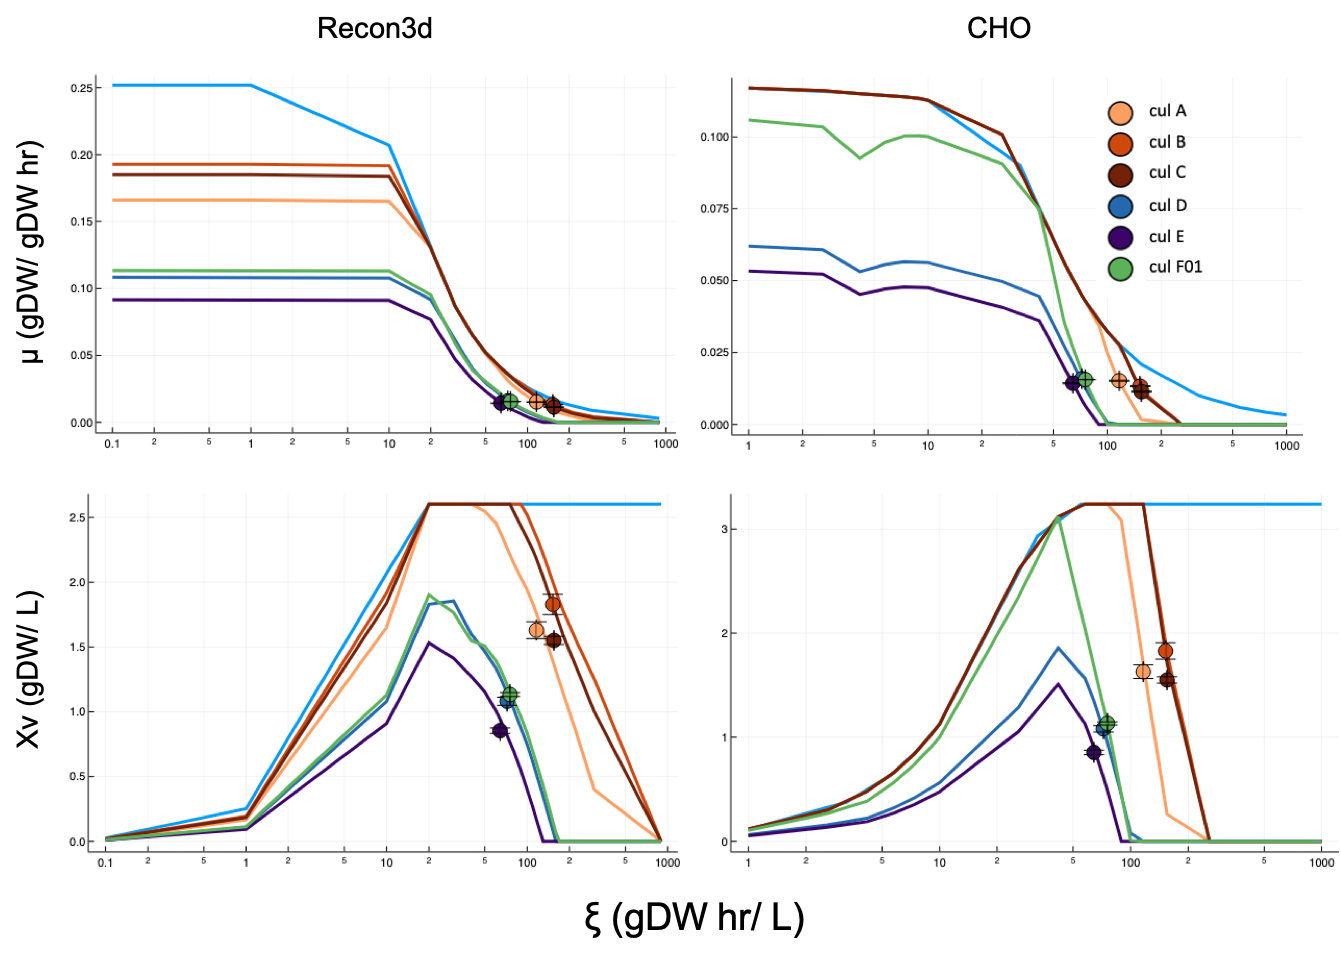
\includegraphics[scale = 0.5]{rich_medium_1}
		\caption{$EP$ and $FBA$ results showing the growth rate, $\mu$, and the viable cell density, $Xv$, dependence of $\xi$ for the six culture conditions. The solid lines represent the model predictions and the color points show the experimental results. $FBA$ results are shown as the solid light blue line. $EP$ $\beta$ parameters was chosen, for each culture, so that the experimental $\mu$ coincides with the modeled one}
		
	\end{figure}
 	
 	This time, additionally to $FBA$, the expected propagation ($EP$) algorithm was used to introduce a population heterogeneity factor \shortcite{Fernandez-de-Cossio-Diaz2018b}. $Figure\ 3$ shows the results of both methods for $Recon3D$ and $CHO$. As can be appreciated, FBA (lite blue solid line) overestimate the experimental results. This is consistent with the fact that we put a carbon source, $PE$, in a high concentration, allowing the network to reach higher $\mu$ and $Xv$ values.
 	
 	 	\begin{figure}[H]
		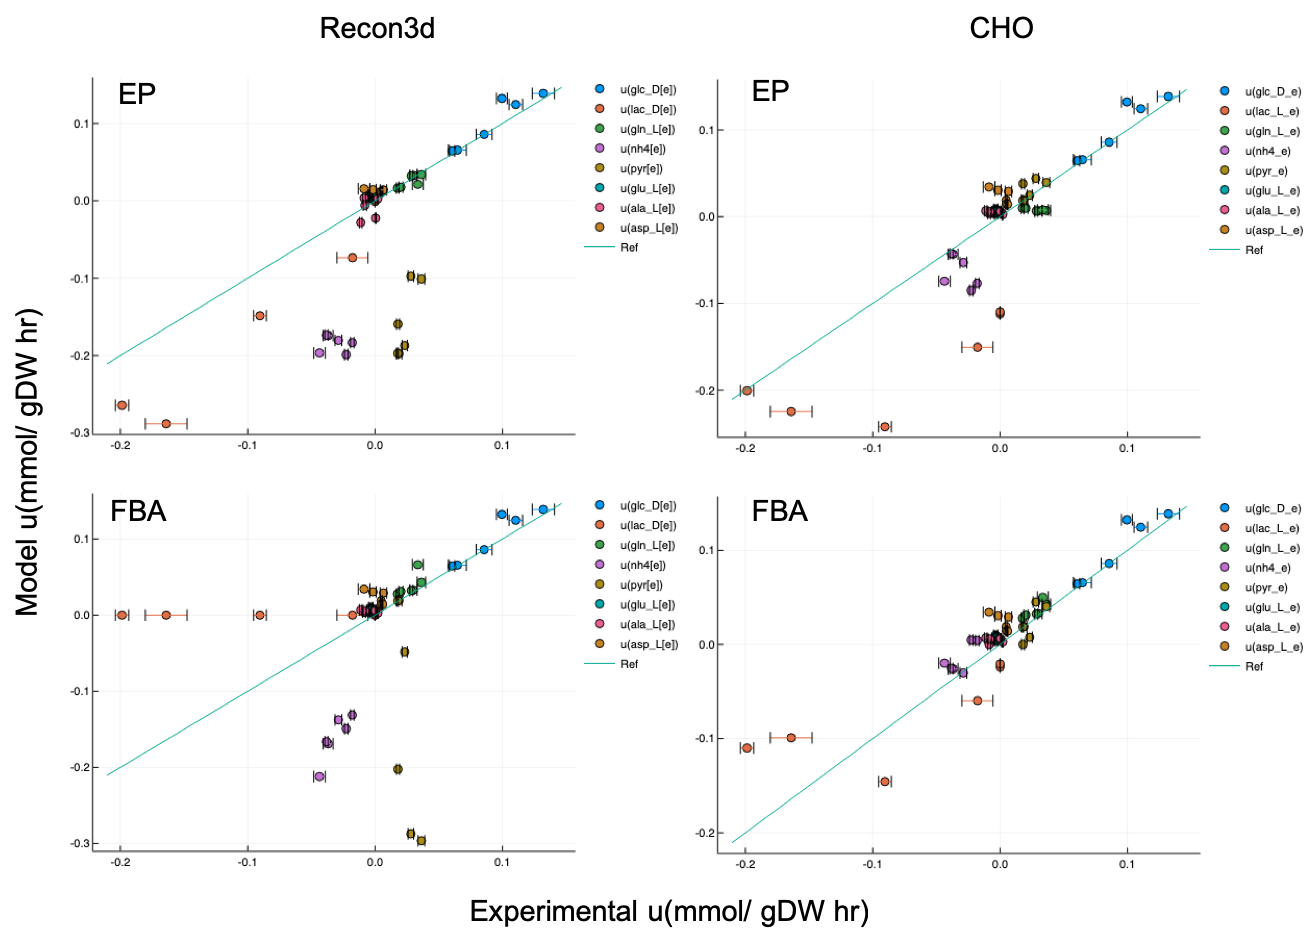
\includegraphics[scale = 0.5]{rich_medium_2}
		\caption{Correlations of all the experimental uptakes compared with the predicted value from $EP$ and $FBA$ for $GEMs$ with 20mM concentration of phosphatidylethanolamine.}
		
	\end{figure}


 	
  	On the other hand, $EP$ can be tuned through parameter $\beta$. This parameter can be interpreted as a measurement of the cell heterogeneity in the culture \shortcite{Fernandez-de-Cossio-Diaz2018b}. $\beta$ values closer to zero indicate higher heterogeneity in the culture, or that the cells can explore more uniformly the space of possibles metabolic states. By contrast, larger $\beta$ values will be approaching the $EP$ model result to $FBA$ result, meaning that no cell heterogeneity is accounted at all. As is appreciated in $Figure\ 3$, considering different $\beta$ values allow the $EP$ model to reproduce the measured $\mu$ and $Xv$. This is an interesting result for several reasons. First, it improves the $FBA$ solution. $FBA$ is insensible to the different experimental conditions, as shown in $Figure\ 1\ and\ 3$. This means that it does not vary the observable predictions, mainly $Xv$, after changing the particular culture conditions, metabolite feed medium concentrations and dilution rate. This occurs for both situations, low and high concentration of $PE$, at least with this $GEM$s and settings. This could, maybe, be explained because $FBA$, as used in this work, returns an optimal metabolic state that maximizes $\mu$. However, it is possible that many different states maximize $\mu$, a not unique solution scenario, and this can make the network robust enough to be insensible to the changes in the input. 
  	
  	Because $EP$ introduces the heterogeneity factor, a better exploration of the space of feasible metabolic states is now possible. There are many factors that can influence the heterogeneity of a population of cells \shortcite{Elowitz2002, Tzur2009, Huh2011, Delvigne2014, King2016, Wang2016, Gonzalez-Cabaleiro2017,  Fernandez-de-Cossio-Diaz2019}. The experimental results can be then interpreted, not only because different input conditions lead to an unique different metabolic state, but because these same changes in the input modified the likelihood distribution of the feasible metabolic states through the cell population. This interpretation is qualitatively different from what $FBA$ represents.
	
  	Furthermore, the correlation of experimental and modeled uptakes was performed, $Figure\ 4$, for both methods. Again, the best correlations were achieved for the uptakes of $GLC$ and $GLN$. A small improvement in the general results can be observed for $EP$ compared with $FBA$, in particular for $Recon3D$. The causes that are driven these results could be the same disused in the previous section. 